\documentclass[12pt]{article}        

\usepackage{fontspec}
\setmainfont{Times New Roman MT Std}
\setmonofont{Times New Roman MT Std}
\usepackage[margin=1in]{geometry}

\usepackage[backend=biber,isbn=false]{biblatex-chicago}
\addbibresource{bibliography.bib}

\usepackage{pdfpages}

\title{Onward: \\ Bringing Finger-Style Guitar to Other Universities}
\author{Rachael Carlson}
\date{\today}

\begin{document}

\maketitle        

\section{Introduction}
\label{sec:introduction}
The world of finger-style is faced with a beautiful problem: there is
currently only one university program in the world which offers a
bachelor's level degree in finger-style guitar. It is beautiful
because there is a program which has the foresight to offer a
program. It is a problem because the fate of finger-style guitar in
the university is intimately intertwined with the success of this
program and its graduates. From an extreme viewpoint, this program
could be viewed as either the catalyst for the flourishing of
finger-style in the university or the death knell for finger-style
guitar. The intention of this paper is to establish a foundation upon
which a proposal for a similar finger-style guitar program at a
university can be built. This proposal can take many forms. I will be
examining numerous possibilities for how a proposal could be constructed.

This topic is massive. This paper is a personal journey and it can be
reflected in the language used in this paper. I am not going to be
able to address each detail of a proposal to a university. While
conducting the research for this paper, my aims shift, my tactics
change. For instance, after speaking with Michael Chapdelaine, my
vision of the future has changed. I plan on redoubling my efforts as a
performer/composer as my avenue by which I may enter academia as a
finger-style guitar instructor. Such changes as this are not to be
viewed as hindrances to the completion of a paper. They are deeply
related to the purpose of this paper.

\section{Tactics}
\label{sec:tactics}
This section will examine the different manners in which it seems, to
me at least, that I might be able to convince a university to offer or
reveal the importance of offering an undergraduate degree in
finger-style guitar performance. The first is to situate the
instrument and its manner of performance within its contexts as a way
to show the historical significance of the style. Second, I will
attempt to look at how the style is existing in the present and how it
might exist in the future as a way to anticipate its future
successes. Finally, and perhaps most importantly, I will discuss
different ways in which I can development as a performer, composer,
and scholar as a means to establish my own significance in relation to
the style. I deem these to be tactics which I should have in my back
pocket, if you will, in case I am ever in a situation in which I might
need to demonstrate the significance of the style or of myself.
\subsection{Situation}
\label{sec:situation}
This tactic takes two forms: first, the history of the guitar; second,
the history of finger-style guitar as a genre of music. I will not
spend too much space in this paper going into a detailed history of
either of these subjects.

The purpose of situating the guitar within its contexts serves
multiple purposes. First, it reinforces my own understanding of and
abilities to discuss the historical components of finger-style guitar
as a manner of playing the instrument and as a genre. Second, this is
an area in which the scholarship is not as robust as it could be: the
history of finger-style guitar is yet to be written. Third, deep
knowledge of these subjects may aid in the pursuit of revealing the
significance of finger-style to individuals who do not know anything
about the guitar or finger-style in particular.

\subsubsection{The History of the Guitar}
\label{sec:history-guitar}
This section of the situation tactic will go into detail on the
development of the steel-string six-string guitar along with an
examination of its predecessors, the seemingly mythic \emph{guitarra
  latina}, the renaissance guitar, the vihuela, the baroque guitar,
and the early six-string guitar. This section would be similar in
focus and breadth to the Finger-Style Guitar: History \& Performance
class offered at the University of Wisconsin-Milwaukee by John
Stropes.
\subsubsection{The History of Finger-Style Guitar}
\label{sec:history-finger-style}
This is one of most exciting areas of interest to me as a scholar. A
history of finger-style guitar has not been written as of the writing
of this paper. I have been formulating theories on how to discuss the
history of finger-style guitar. The most convincing way, to me, to
discuss the history borrows from studies on feminism.\footnote{It
  appears that Martha Lear of \emph{The New York Times} was the
  individual who coined the term `first-wave feminism.'} In the
historiographies of feminism, authors frequently use the term `wave'
to describe groups of contemporaneous feminists (i.e. 1st wave
feminists, 2nd wave, etc.). In the case of finger-style guitarists, I
believe that the history would begin with proto-finger-style
guitarists who could be considered the first wave. These
proto-finger-style guitarists would be individuals such as Arthur
`Blind' Blake, Huddie `Leadbelly' Ledbetter, Charlie Patton, Lonnie
Johnson, Robert Johnson, Maybelle Carter, and others who were playing
the guitar with their fingers and not a plectrum during this era. If I
were to produce a paper on this subject, I would most likely start by
limiting the scope to the history of finger-style guitar as a genre in
the United States. Even limited the scope to finger-style guitar as a
genre might suffice.\footnote{The plectrum-style compositions of
  Michael Hedges propose a curious case in this respect. Perhaps not
  dissimilar to proto-finger-style guitar compositions such as
  ``Guitar Chimes'' by Blind Blake, plectrum-style compositions by
  notable finger-style guitarists could be considered finger-style in
  an honorary sense.} It is important to understand one's historical
contexts. It is from these perspectives that one might be able to
anticipate future developments of the genre.

\subsection{Projection}
\label{sec:projection}
I see this tactic as having two subsections, the near-present and
possible futures. The near-present would examine the changing
landscape of the business of music. More specifically, I would attempt
to find some numbers, real data, on the presence of finger-style
guitar on YouTube and other internet sites as a way to establish the
ubiquity of finger-style guitar. This information would help project
the status of finger-style in the future.  The goal of this research
would be reinforce my perspective toward the future in a way that I
can energize those around me to the unique possibilities of offering a
finger-style guitar performance degree.
\subsection{Personal Growth}
\label{sec:personal-growth}
After the interview with Michael Chapdelaine in which he said that he
thought that I would need a D.M.A. in order to be hired as a
tenure-track faculty member in guitar performance, the personal growth
tactic become much more important to me. I realized that Chapdelaine
might have been referring to classical guitar instruction in relation
to his recommendation of a D.M.A. This leads me to believe that one
way into academia as a finger-style guitar instructor could be through
establishing myself as a performer and composer within the genre. This
could perhaps fulfill an experiential requirement for employment.
\subsubsection{As a Composer}
\label{sec:composer}
A marker of success in the world of finger-style guitar as a genre is
the performer as composer. The artists who are success who do not
compose are in the minority. Their number can be counted on one
hand. The finger-style guitarist as composer is a unique component of
finger-style guitar. This generative characteristic of finger-style
guitarists is one of the major characteristics which sets it apart
from classical guitar.

I have taken private lessons in composition. I have received several
recommendations for books which aim to assist in the composition
process. One such book, recommended by Dr. Monhardt, is \emph{Learning
  to Compose} by Larry Austin and Thomas Clark.\autocite{austin1989}
This book is out of print, with used copies frequently selling for
more than \$200. I have a copy from the university library which I
will copy before I need to give it back to the library. Another
recommendation, this time from Dr. Heinrichs, is \emph{Musical
  Composition} by Reginald Smith Brindle.\autocite{brindle} This book
is easily available through book retailers with used copies selling
for less than \$20.

In the next several months I will compose enough music to record an
album of original finger-style guitar music. Once I reach this point,
I will send my music around to various record labels to determine
interest in my work. Record Labels of interest include: Candyrat
Records, Righteous Babe Records, Constellation Records, and ECM
Records, to name a few.\autocites{candyrat,righteous} Knowing that
there is a possibility that none of the above labels will show
interest in my work, I will figure out what is necessary to
independently produce the record in order to continue my career as a
performer.

\subsubsection{As a Performer}
\label{sec:performer}
I have worked diligently in Milwaukee to establish myself as a
performer of finger-style guitar music. I believe that in the last ten
years I have made a name for myself in Milwaukee. I have opened for
Don Ross and David Wilcox. I have played at the Milwaukee LGBT Film
Festival opening reception three years in a row at the Villa
Terrace. I had a weekly gig playing music for the dinner crowd on
Wednesdays at Centro, an Italian restaurant in Milwaukee's Riverwest
neighborhood. I have played for various functions at UWM as a
performer recommended by the Dean of Peck School of the Arts. As part
of my degrees in performance, I have given three recitals as a solo
finger-style guitarist. As a member of an ensemble, I have played for
the Florentine Opera and in the progressive rock band \textsc{sun rock
  man}. As a lutenist I have played basso continuo with Camerata
Milwaukee and fundraisers for Early Music Now.

I will be moving to Boise, Idaho at the end of May, 2017. I currently
have one gig in Boise; I will be playing guitar and banjo in a
production of the musical \emph{Oklahoma!}. I have several goals, in
no particular order, as a performing musician in Boise: first, find as
many gigs in the area as possible; second, compose an album's worth of
material; third, identify and begin working on beginning finger-style
guitar repertoire with the aim of establishing a larger core of
material for the development of finger-style guitar performers;
fourth, establish a regimen of physical fitness which will help
improve my ability to perform all of the above.

\subsubsection{As a Scholar}
\label{sec:scholar}
This component of personal growth was discussed briefly above. I
believe that it is possible to find a niche within the field of
ethnomusicology with a study of the history of finger-style guitar as
a genre of music. A published article in a scholarly journal can only
assist in garnering a position in finger-style guitar instruction. I
would imagine that there are few guitar instructors at an institution
of higher education who also have published articles in scholarly
journals. 
\section{Interviews}
\label{sec:interviews}
I wanted to discuss some of the issues that we face as academic guitar
players with individuals who include finger-style guitar in their
curricula as guitar instructors are universities or colleges. I found
four individuals who do such a thing: Michael Millham of Gonzaga
University and Eastern Washington University; Michael Chapdelaine of
University of New Mexico; Sean McGowan of University of Colorado at
Denver; and John Stropes of University of Wisconsin-Milwaukee. I was
able to interview Millham and Chapdelaine. These were the first steps
taken to construct a bridge between UWM's finger-style guitar program
and other universities in the country. I was unable to interview John
Stropes and Sean McGowan. The aim with the interviews was to determine
how the instructor interacted with finger-style guitar in their
respective positions and to determine a best course of action for an
individual who is interested in teaching finger-style guitar at a
college or university. I have included transcripts of the interviews
with the submission of this paper.

Michael Millham teaches only guitar majors at Eastern Washington
University. At Gonzaga University, he teaches mostly music education
students. In the interview Millham, indicated that the degrees that
are offered by Eastern Washington University are flexible enough that
if a student wanted to pursue a BA in Guitar Performance with an
emphasis on finger-style guitar. This university is able to use ``that
secondary holder as a catch-all for people who don't want to do the
lute suites.''\footnote{Michael Millham, interview with the author on
  May 11, 2017, University of Wisconsin-Milwaukee, Milwaukee, WI. Page
  8 of attached transcript.} At Gonzaga, he has some performance
students. Millham was not very clear about exactly how finger-style
guitar interacted with his institution.

Millham in discussing advice for a finger-style guitarist who would be
interested in teaching at the college-level recommended that
\begin{quote}
  if somebody can play well, and they get well known in a town that
  does not have a guitar program \emph{and} they have the piece of
  paper, then pitching the [unintelligible] guitar program. And then,
  once you get in you can teach what you want. Why not teach a
  finger-style program? It sounds cool.\footnote{Michael Millham,
    interview with the author on May 11, 2017, University of
    Wisconsin-Milwaukee, Milwaukee, WI. Page 10 of attached
    transcript.}
\end{quote}
Millham's interview was marked by a sense of optimism for the future
of guitar studies in spite of the trends in university business
structure to higher workers by using the ``temp worker'' model. A
distillation of this idea can be stated by Millham thus: ``This idea
that a degree will buy you a job is false. Your skill and your
attributes buy you a job and your degree is an envelope to package it
in, in my opinion.''\footnote{Michael Millham, interview with the
  author on May 11, 2017, University of Wisconsin-Milwaukee,
  Milwaukee, WI. Page 11 of attached transcript.}

Michael Chapdelaine has a storied history within the world of
classical guitar. He indicated that he had difficulties when first
hired to work as a tenure-track faculty member of the University of
New Mexico's guitar department. He has mostly taught classical guitar
at this level. However in the past few years he notes that its ``been
growing a lot…because I just took the reins off of the
curriculum.''\footnote{Michael Chapdelaine, interview with the author,
  April 29, 2017, University of Wisconsin-Milwaukee, Milwaukee,
  WI. Page 4 of attached transcript.} Chapdelaine notes that he has
two years of programmed, classical study of the guitar. Once the
student has progressed past this Michael asks the student ``what do
you want to play?''\footnote{Ibid., 6.} If a student wants to play
finger-style guitar Chapdelaine assists them in that
endeavor. Chapdelaine's recommendation to students interested in
teaching at the college-level is that he or she needs at least a DMA
in classical guitar performance in order for a university to consider
the application. Chapdelaine's approach to finger-style guitar is very
similar to his approach to classical guitar. He considers it all to be
``polyphonic guitar music.''\footnote{Ibid., 7.}

There is a lot to consider in these interviews. I would charge the
reader with carefully reading the transcripts of these
interviews. They are two very different personalities and viewpoint on
and in the pedagogy of guitar. Personally, there is a lot to consider
as well. I can't help but want to side with Millham's recommendations
as I have little interest in going back to school for a DMA in
classical guitar performance.

\section{Conclusions}
\label{sec:conclusions}
Much of the work that I have done in this master's degree has been
preliminary work. This paper is no exception. It is the beginning of a
career in guitar performance and instruction. I hope that the
excitement that I feel about this subject is apparent in these
pages. I feel that I have a better understanding of how I can continue
as a finger-style guitarist in the 21st century through the work that
I have done for this degree.
\clearpage
\printbibliography
\clearpage
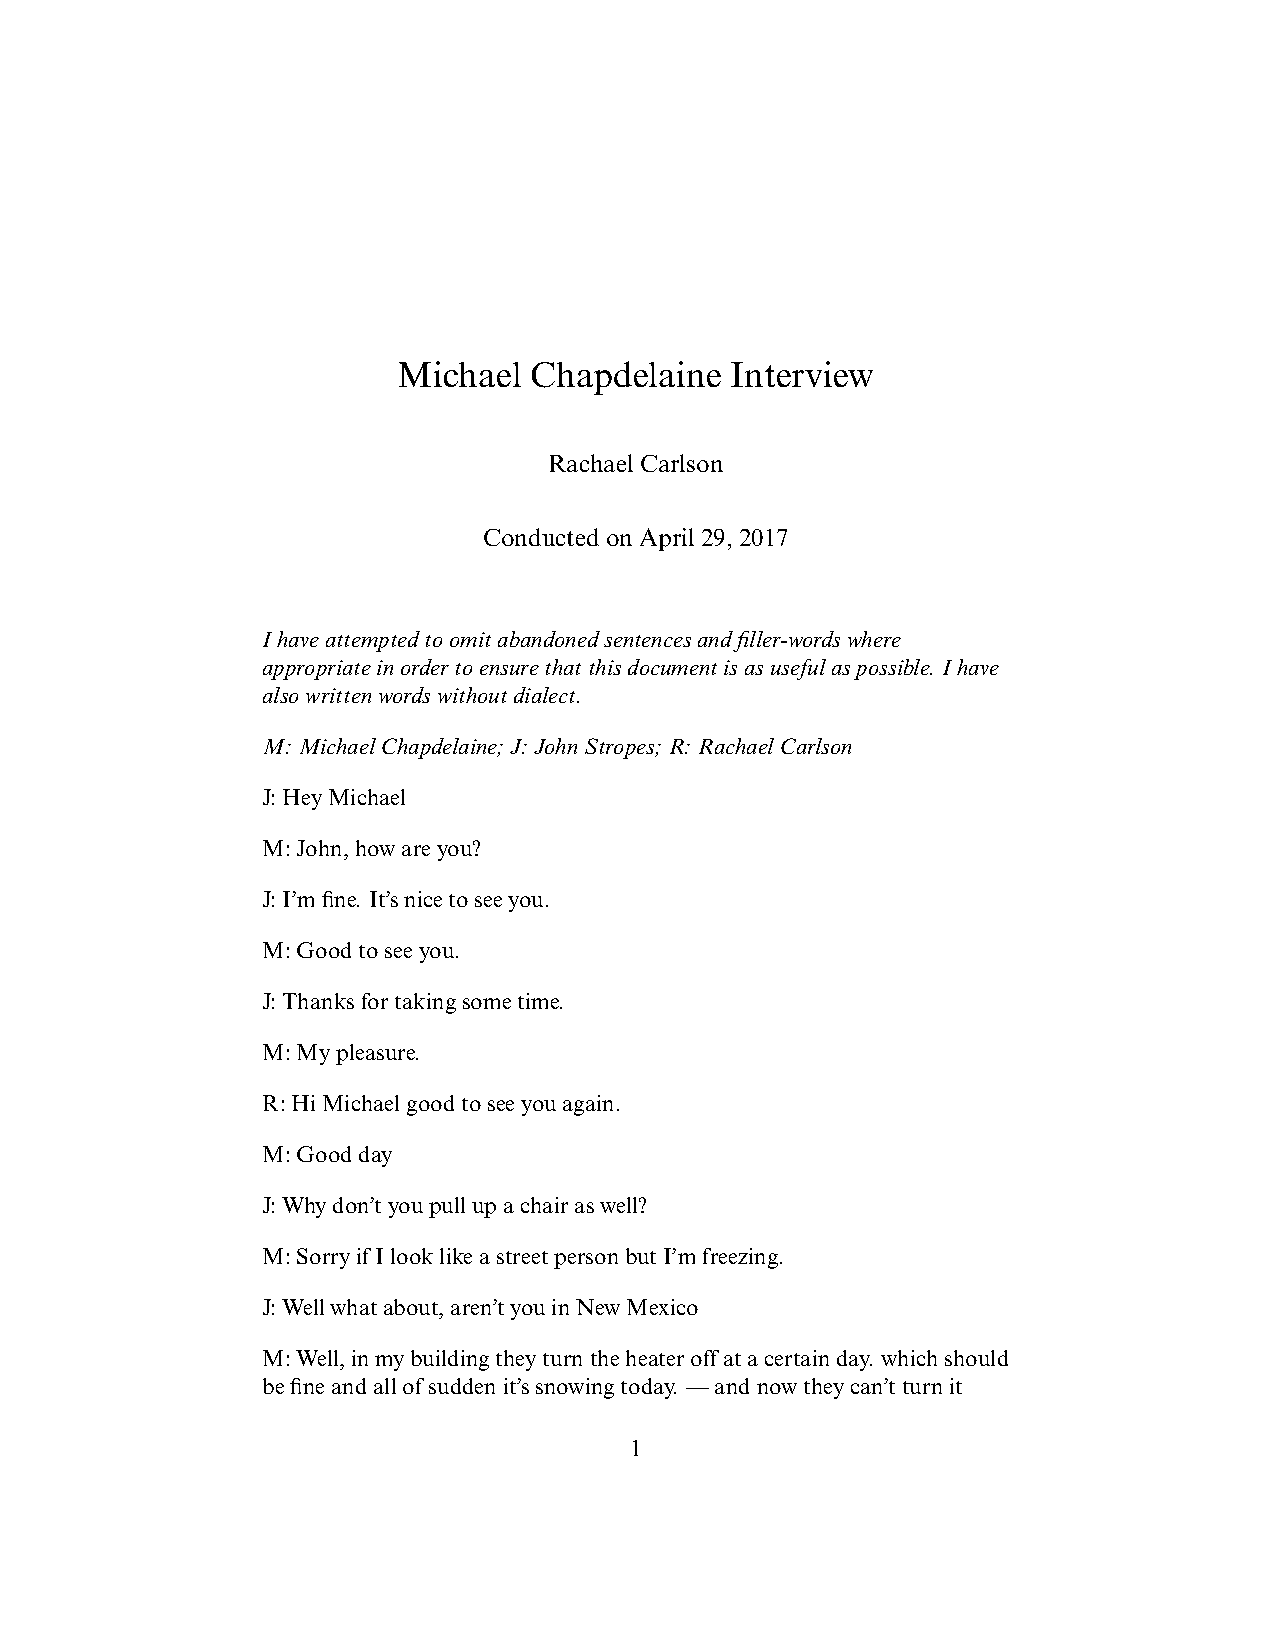
\includepdf[pages=-,pagecommand={}]{Interviews/Chapdelaine/MichaelChapdelaineInterview.pdf}
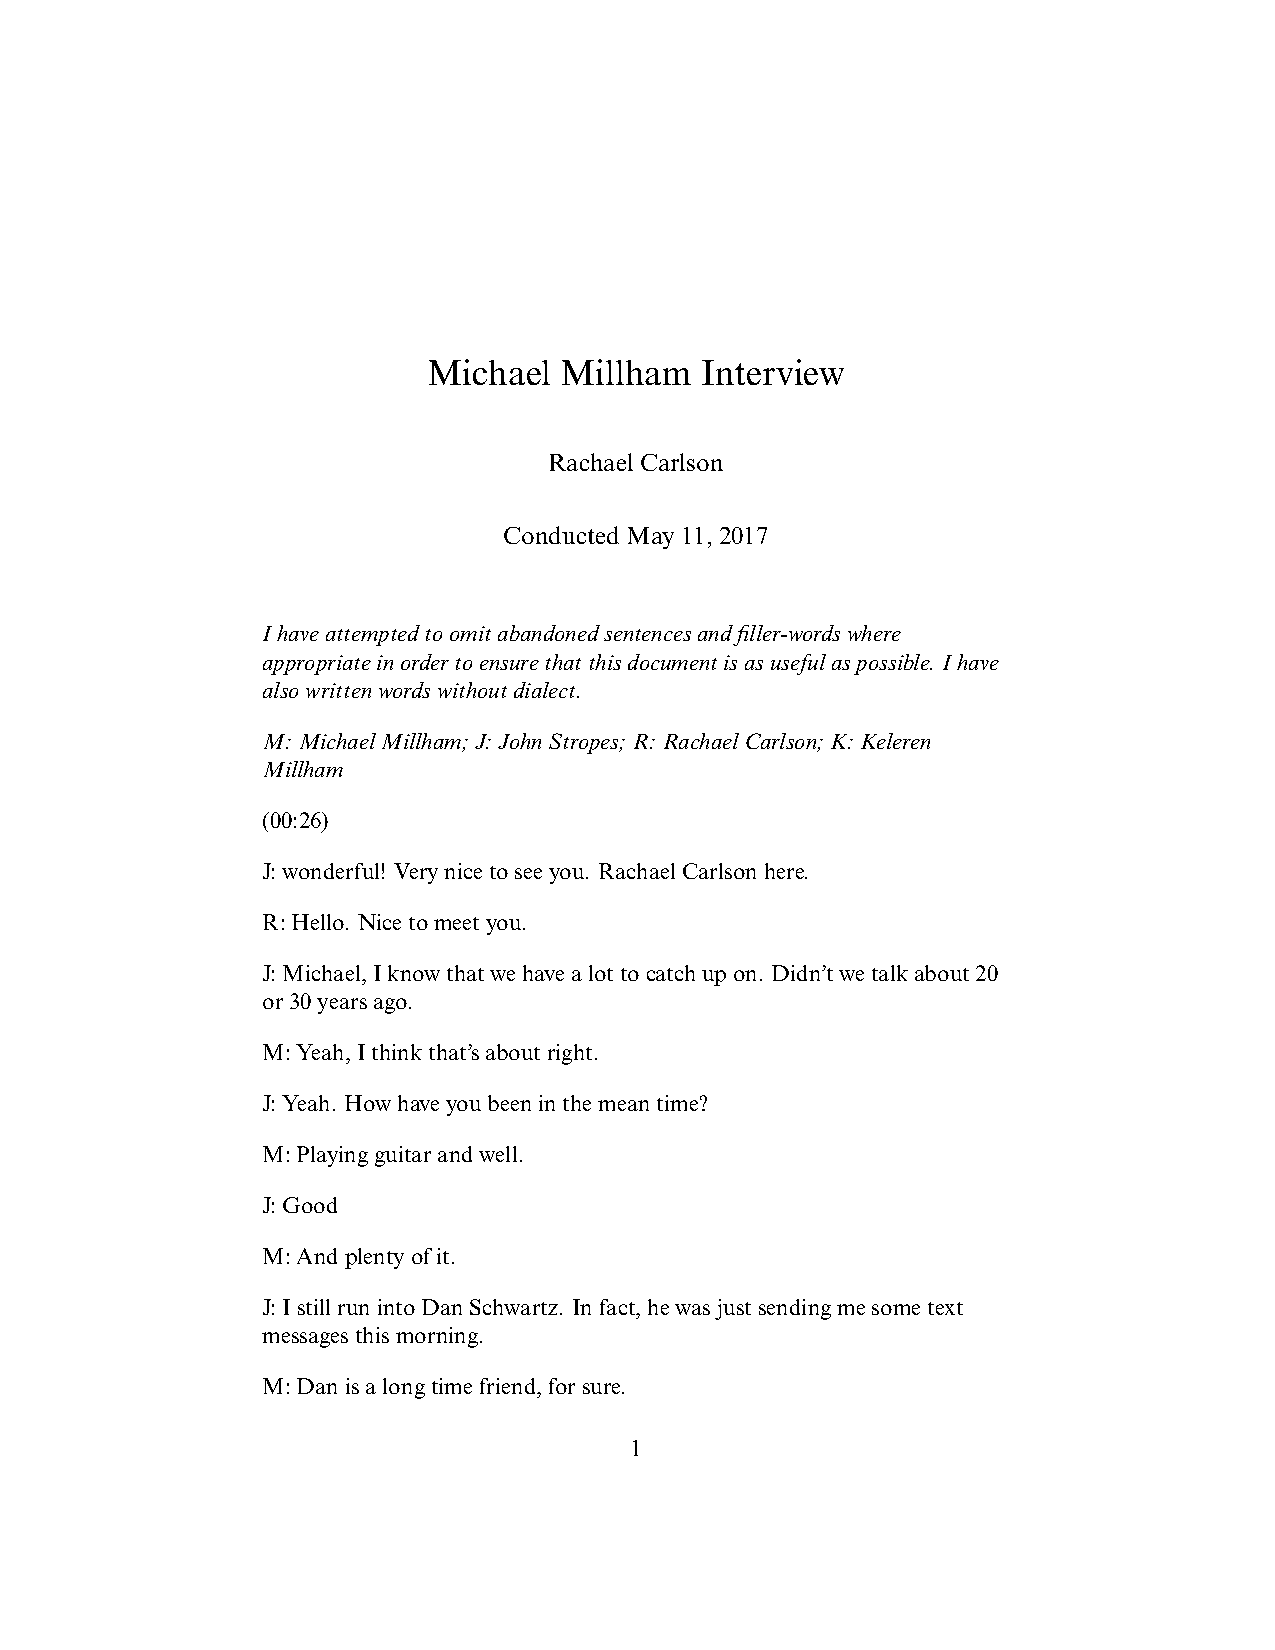
\includepdf[pages=-,pagecommand={}]{Interviews/Millham/millhamInterview.pdf}
\end{document}
%%% Local Variables:
%%% mode: latex
%%% TeX-master: t
%%% End:
